\subsection{The I-prior probit model}
\begin{frame}{The I-prior probit model}
  \begin{tikzpicture}[scale=1.1, transform shape]
    \tikzstyle{main}=[circle, minimum size = 10mm, thick, draw =black!80, node distance = 16mm]
    \tikzstyle{connect}=[-latex, thick]
    \tikzstyle{box}=[rectangle, draw=black!100]
      \node[main, draw=none] (fake) {};
      \node[main, fill = black!10] (H) [right=of fake, xshift=-1.65cm] {$x_i$};
      \node[main, double, double distance=0.6mm] (eta) [right=of H] {$f_i$};
      \node[main, double, double distance=0.6mm] (ystar) [right=of eta] {$p_i$};
      \node[main, draw=colblu] (lambda) [above=of H, xshift=0.4cm, yshift=-0.4cm] {\color{colblu} $\lambda$};  %
      \node[main, draw=colgre] (alpha) [above=of eta, yshift=0.3cm] {\color{colgre} $\alpha$};  
      \node[main, fill = black!10] (y) [right=of ystar] {$y_i$};
      \node[main, draw=colred] (w) [below=of eta, yshift=0.4cm] {\color{colred} $w_i$};  
      \path (alpha) edge [connect] (eta)
            (lambda) edge [connect] (eta)
    		(H) edge [connect] (eta) 
    		(eta) edge [connect] node [above] {$\Phi$} (ystar)
    		(ystar) edge [connect] (y)
    		(w) edge [connect] (eta)
            (H) edge [] node [above] {$h$} (eta);
      \node[rectangle, draw=black!100, fit= (H) (y) (w) ] {}; 
      \node[rectangle, fit= (w) (y), label=below right:{$i=1,\dots,n$}, xshift=-0.35cm, yshift=0.55cm] {};  % the label
    \end{tikzpicture}
    
    \begin{textblock*}{0.48\textwidth}(0.52\textwidth,0.55cm)
    \begin{block}{}
    \vspace{-1.6em}
      \begin{align*}
        &p(\by,\bw,\alpha,\lambda)  \\
        &= p(\by|\bff)p(\bw)p(\lambda)p(\alpha) \\
        &= {\textstyle\prod_{i=1}^n} \Phi(f_i)^{y_i} \big(1 - \Phi(f_i)\big)^{1-y_i} \\
        &\phantom{==} \cdot {\color{colred} [\N(0,1)]^n} 
        \cdot {\color{colblu} \N(\lambda_0,\kappa_0^{-1})} \\
        &\phantom{==} \cdot {\color{colgre} \N(\alpha_0,\tau_0^{-1})}
      \end{align*}
    \end{block}
  \end{textblock*}
\end{frame}

\subsection{Laplace's method}
\begin{frame}[label=laplace]{Laplace's method}
  \blfootnote{\fullcite[§4.1, pp.777-778.]{Kass1995}}
  \vspace{-15pt}
  \begin{itemize}[<+->]\setlength\itemsep{0.8em}
    \item Interested in $p(\bff|\by) \propto p(\by|\bff)p(\bff) =: e^{Q(\bff)}$, with normalising constant $p(\by) = \int e^{Q(\bff)} \d\bff$. The Taylor expansion of $Q$ about its mode $\tilde\bff$
    \[
      Q(\bff) \approx Q(\tilde\bff) - \half (\bff - \tilde\bff)^\top\bA(\bff - \tilde\bff) 
    \]
    is recognised as the logarithm of an unnormalised Gaussian density, with $\bA = -\text{D}^2 Q(\bff)$ being the negative Hessian of $Q$ evaluated at  $\tilde\bff$.
    \item The posterior $p(\bff|\by)$ is approximated by $\N(\tilde\bff, \bA^{-1})$, and the marginal by
    \[
      p(\by) \approx (2\pi)^{n/2} \vert \bA \vert^{-1/2}  p(\by|\tilde\bff)p(\tilde\bff)
    \]
    \item Won't scale with large $n$; difficult to find modes in high dimensions.
  \end{itemize}
  
  \begin{textblock*}{3cm}(.982\textwidth,1.04\textheight)%
    \hyperlink{estimation}{\beamerbutton{back}}      
  \end{textblock*}
\end{frame}

\subsection{Full Bayesian analysis of I-probit models}
\begin{frame}[label=mcmc]{Full Bayesian analysis using MCMC}
  \vspace{-3pt}
  \begin{itemize}\setlength\itemsep{0.5em}
    \item Assign hyperpriors on parameters of the I-prior, e.g.
    \begin{itemize}
      \item $\lambda^2 \sim \Gamma^{-1}(a,b)$
      \item $\alpha \sim \N(c,d^2)$
    \end{itemize}
    for a hierarchical model to be estimated fully Bayes.
    \item No closed-form posteriors - need to resort to MCMC sampling.
    \item Computationally slow, and sampling difficulty results in unreliable posterior samples.
  \end{itemize}
  \begin{center}
    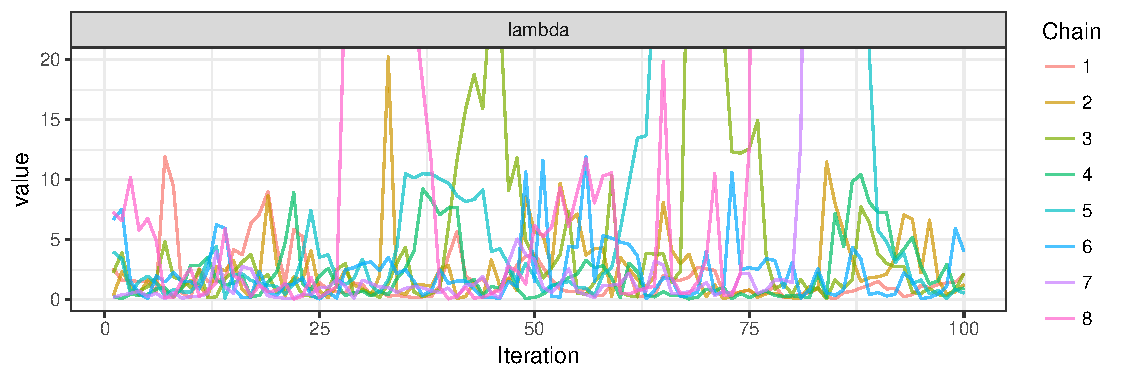
\includegraphics[scale=0.6]{mcmc1}
  \end{center}

  \begin{textblock*}{3cm}(.982\textwidth,1.04\textheight)%
    \hyperlink{estimation}{\beamerbutton{back}}      
  \end{textblock*}  
\end{frame}

\subsection{Variational inference}

\begin{frame}{Variational inference}
  \vspace{-10pt}
  \begin{itemize}[<+->]
    \item Name derived from calculus of variations which deals with maximising or minimising functionals.
    \begin{table}
      \begin{tabular}{l  l  l }
      Functions   &$p:\theta \mapsto \bbR$  &(standard calculus) \\ 
      Functionals &$\cH:p \mapsto \bbR$     &(variational calculus) \\ 
      \end{tabular}
    \end{table}
  \item Using standard calculus, we can solve
  \[
    \argmax_\theta p(\theta) =: \hat\theta
  \]
  e.g. $p$ is a likelihood function, and $\hat\theta$ is the ML estimate.
  \item Using variational calculus, we can solve
  \[
    \argmax_p \cH(p) =: \tilde p
  \]
  e.g. $\cH$ is the entropy $\cH = - \int p(x)\log p(x) \d x$, and $\tilde p$ is the entropy maximising distribution.
  \end{itemize}
  \vspace{5pt}
\end{frame}

\begin{frame}[label=varcompare]{Comparison of approximations (density)}
  \vspace{-5pt}
  \only<1|handout:0>{
    \begin{center}
      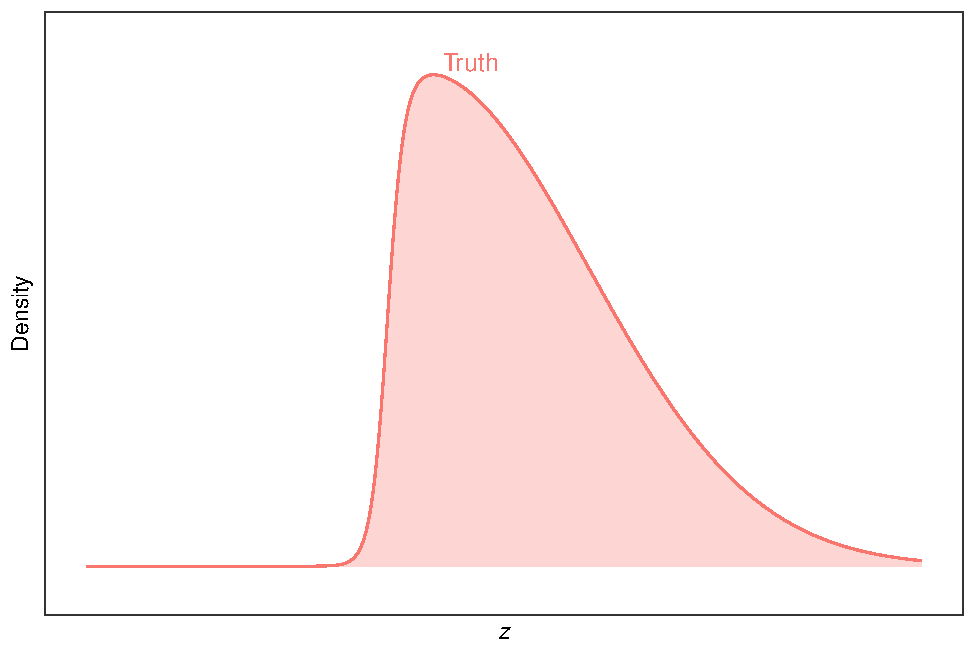
\includegraphics[scale=0.7]{figure/compare1}
    \end{center}
  }
%  \only<2|handout:0>{
%    \begin{center}
%      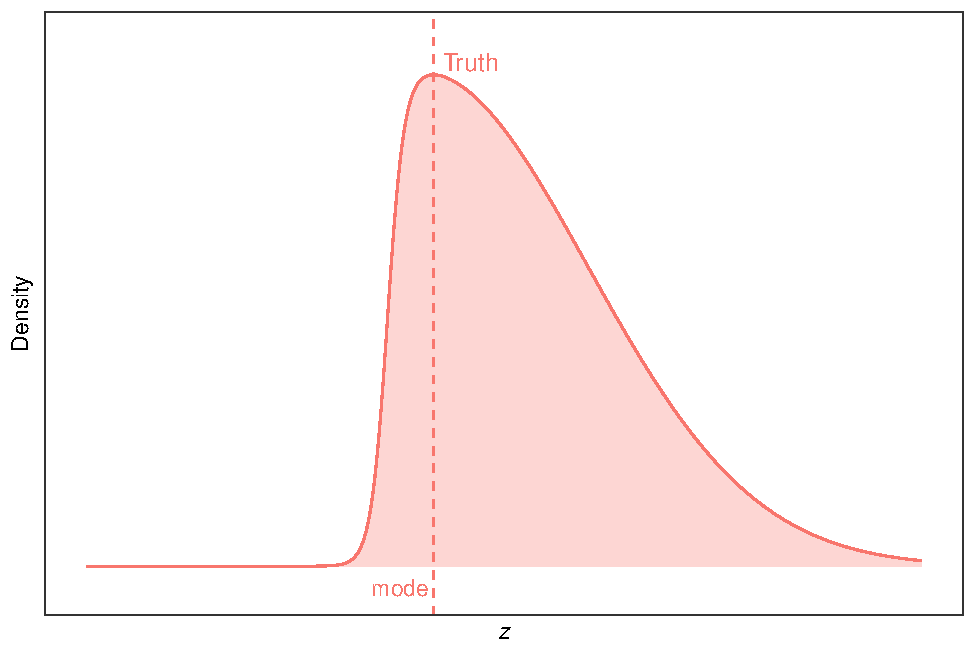
\includegraphics[scale=0.7]{figure/compare2}
%    \end{center}
%  }  
  \only<2|handout:0>{
    \begin{center}
      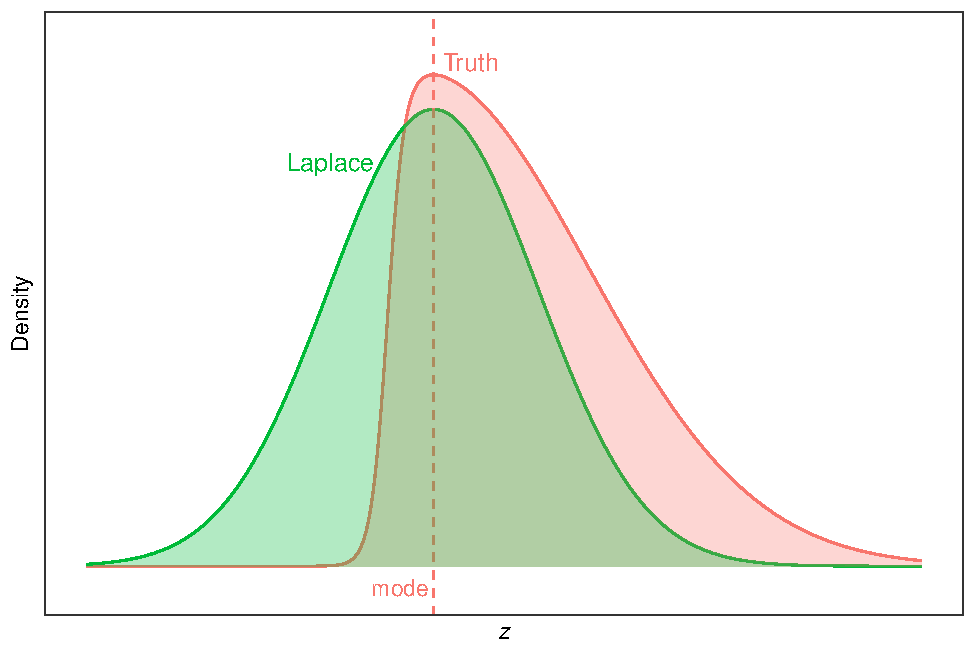
\includegraphics[scale=0.7]{figure/compare3}
    \end{center}
  } 
%  \only<4|handout:0>{
%    \begin{center}
%      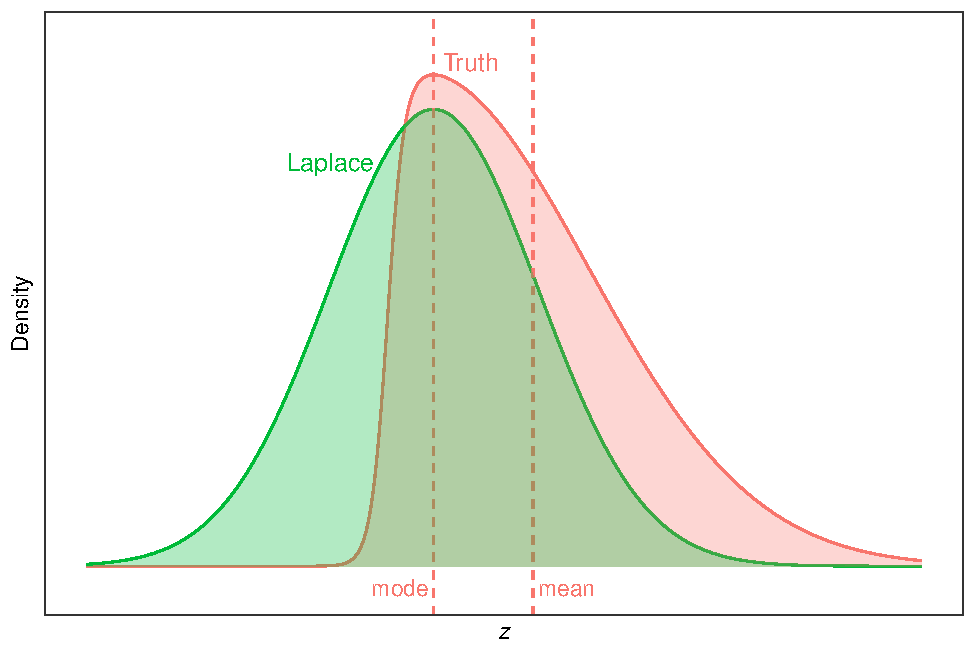
\includegraphics[scale=0.7]{figure/compare4}
%    \end{center}
%  } 
  \only<3|handout:1>{
    \begin{center}
      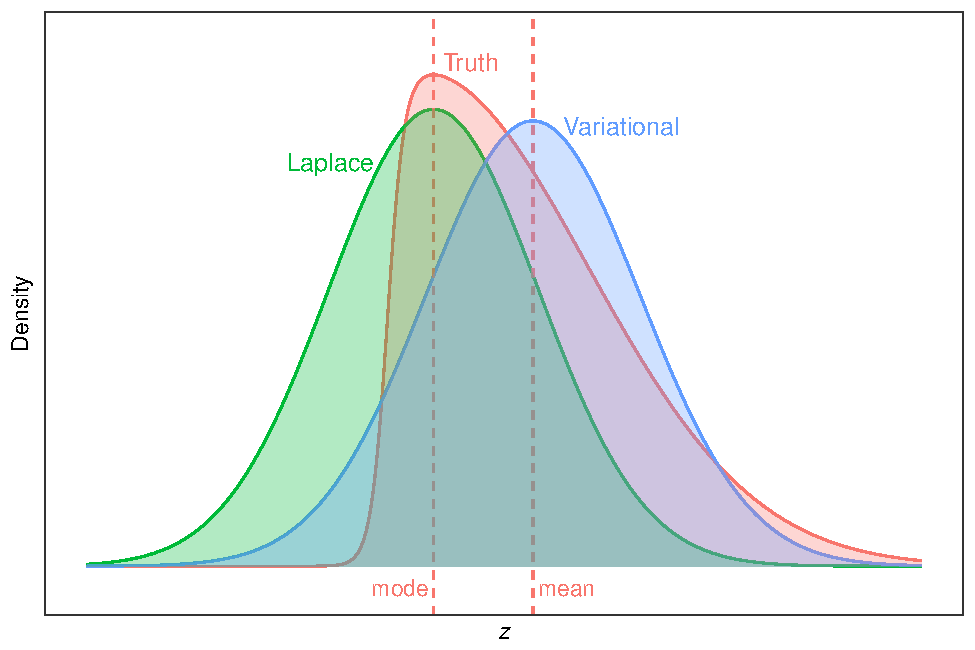
\includegraphics[scale=0.7]{figure/compare5}
    \end{center}
  } 
  
  \begin{textblock*}{3cm}(.982\textwidth,1.04\textheight)%
    \hyperlink{summary}{\beamerbutton{back}}      
  \end{textblock*}
\end{frame}

\begin{frame}{Comparison of approximations (deviance)}
  \vspace{-5pt}
  \begin{center}
    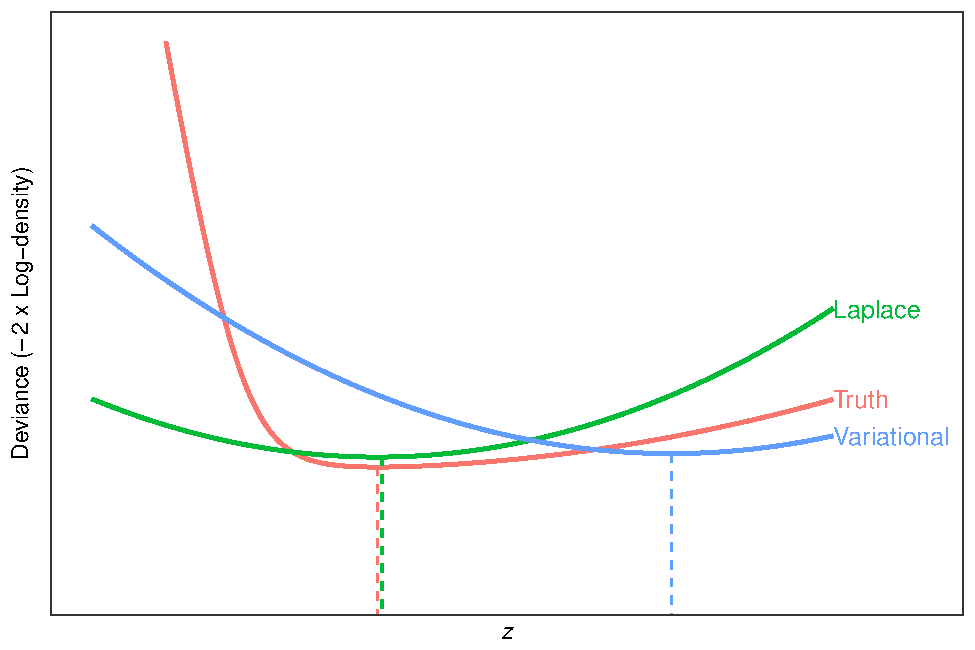
\includegraphics[scale=0.7]{figure/compare6}
  \end{center}

  \begin{textblock*}{3cm}(.982\textwidth,1.04\textheight)%
    \hyperlink{summary}{\beamerbutton{back}}      
  \end{textblock*}  
\end{frame}

\subsection{A simple variational inference example}

\setbeamercovered{still covered={\opaqueness<1->{0}},again covered={\opaqueness<1->{15}}}
\begin{frame}[label=varex]{Estimation of a 1-dim Gaussian mean and variance}
  \vspace{-5pt}
  \begin{itemize}
    \item<1-3> \textbf{GOAL}: Bayesian inference of mean $\mu$ and variance $\psi^{-1}$
    \begin{center}
      {\def\arraystretch{1.2}
      \begin{tabular}{c c l}
        $\displaystyle y_i \iid \N(\mu, \psi^{-1})$ & & Data \\
        {\color{gray!88}$\displaystyle \mu|\psi \sim \N\big(\mu_0,(\kappa_0\psi)^{-1}\big)$} & & {\color{gray!88}\multirow{2}{*}{Priors}} \\
        {\color{gray!88}$\displaystyle \psi \sim \Gamma(a_0,b_0)$} & \\
        $\displaystyle i=1,\dots,n$ & \\
      \end{tabular}
      }
    \end{center}
    \item<2-3> Substitute $p(\mu,\psi|\by)$ with the mean-field approximation
    \[
      q(\mu, \psi) = q_\mu(\mu) q_\psi(\psi)
    \]
    \item<3-> From \eqref{eq:meanfieldsoln}, we can work out the solutions 
    
    \only<5|handout:0>{
    \begin{align*}
      \log \tilde q_\mu(\mu) 
      &= \E_\psi[\log p(\by|\mu,\psi)] + \E_\psi[\log p(\mu|\psi)] + \const \\[0.5em]
    \log \tilde q_\psi(\psi) 
    &= \E_\mu[\log p(\by|\mu,\psi)] + \E_\mu[\log p(\mu|\psi)] + \log p(\psi) \\
    &\phantom{==} + \const
    \end{align*}
    }
    
    \vspace{-3pt}
    \begin{gather*}
      \uncover<6->{
      \hspace{-12pt}\tilde q_\mu(\mu) \equiv \N \left(\frac{\kappa_0 \mu_0 + n\bar y}{\kappa_0 + n}, \frac{1}{(\kappa_0 + n)\E_q[\psi]} \right)}
      \uncover<7->{
      \ \text{ and } \ \
      \tilde q_\psi(\psi) \equiv \Gamma(\tilde a, \tilde b) \\[0.5em]
      \hspace{-12pt}\tilde a = a_0 + \half[n] \hspace{1.1cm} \tilde b = b_0 + \half \E_q\Big[ {\textstyle\sum_{i=1}^n} (y_i - \mu)^2 + \kappa_0(\mu - \mu_0)^2 \Big]
      }
    \end{gather*}
  \end{itemize}
  
  \only<4-|handout:0>{
  \begin{textblock*}{0.8\textwidth}(1.35cm,0.215\textheight)
    \begin{block}{}
      \begin{itemize}
        \item Under the mean-field restriction, the solution to $\argmax_q \cL(q)$ is
        \begin{align*}
          \tilde q_j(\bz^{(j)}) \propto \exp\big(\E_{-j}[\log p(\by,\bz)]\big)
          \rlap{\hspace{1.3cm}(1)}
        \end{align*}
        for $j \in \{1,\dots,m\}$.  
      \end{itemize}
    \end{block}
  \end{textblock*}
  }

  \begin{textblock*}{3cm}(.982\textwidth,1.04\textheight)%
    \hyperlink{cavi}{\beamerbutton{back}}      
  \end{textblock*}

\end{frame}

\begin{frame}{Estimation of a 1-dim Gaussian mean and variance (cont.)}
  \vspace{-5pt}
%  \only<1>{
%    \begin{center}
%      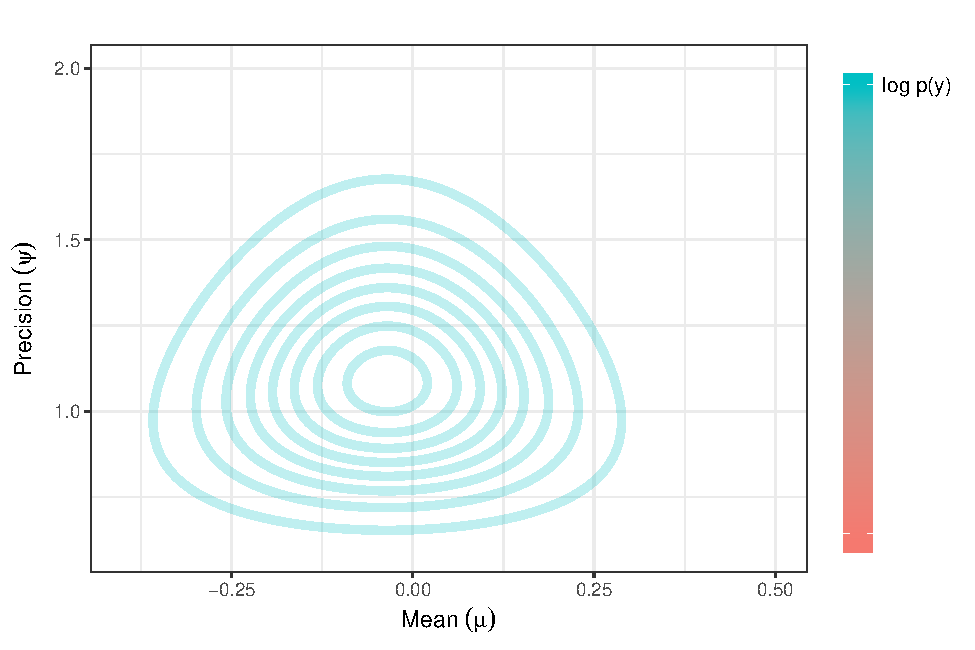
\includegraphics[scale=0.7]{figure/vbupdate}
%    \end{center}
%  } 
  \only<1|handout:1>{
    \begin{center}
      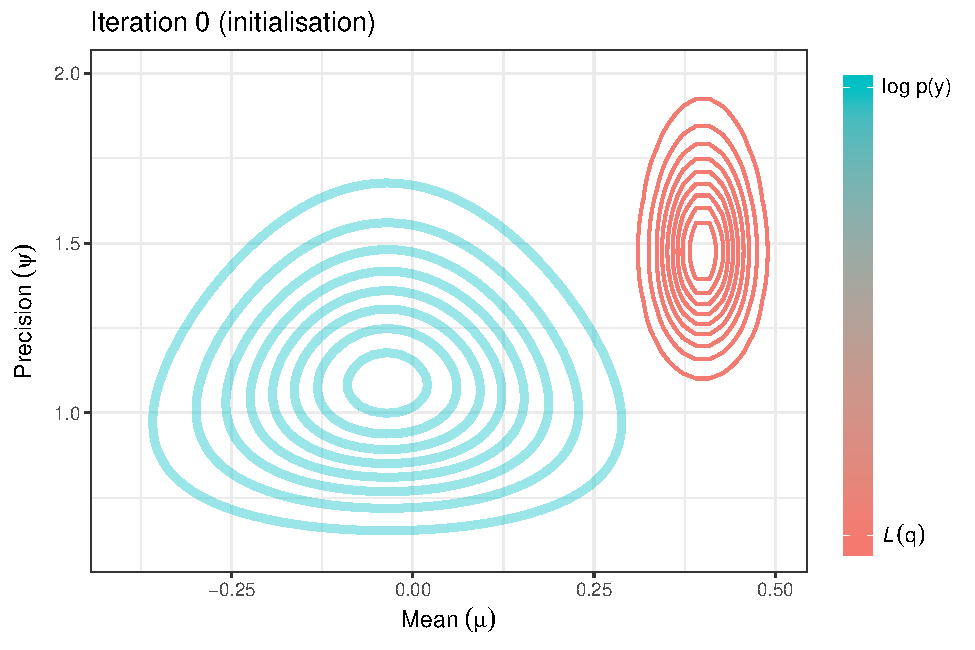
\includegraphics[scale=0.7]{figure/vbupdate_7}
    \end{center}
  } 
  \only<2|handout:2>{
    \begin{center}
      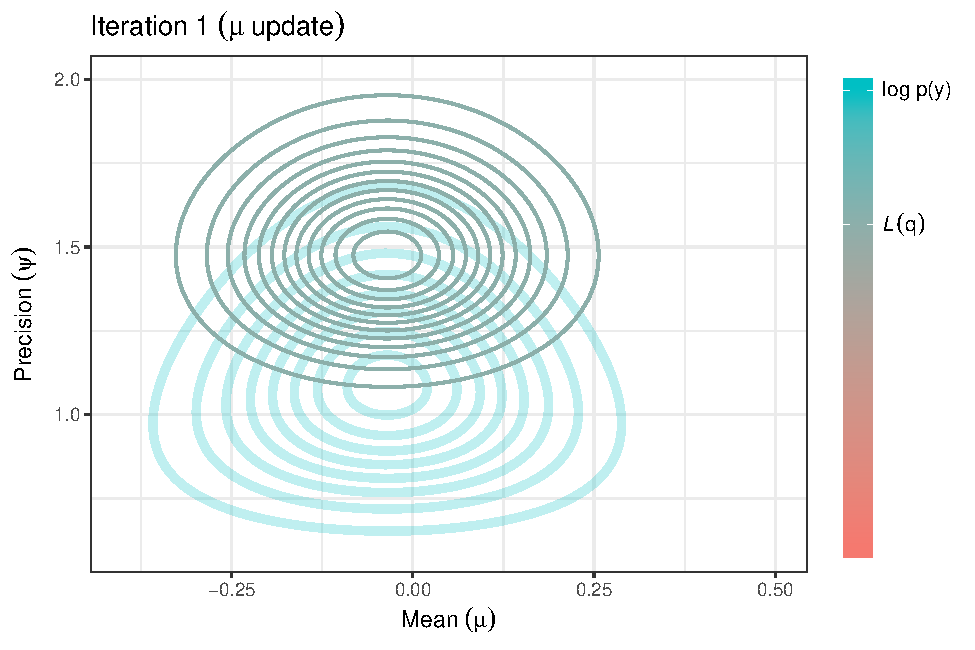
\includegraphics[scale=0.7]{figure/vbupdate_1}
    \end{center}
  } 
  \only<3|handout:3>{
    \begin{center}
      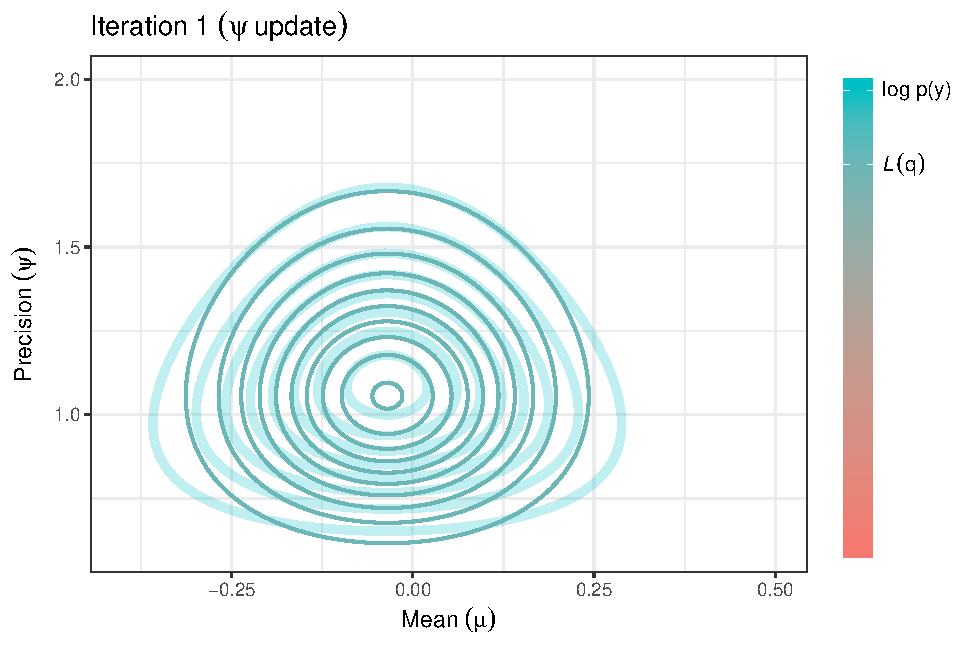
\includegraphics[scale=0.7]{figure/vbupdate_2}
    \end{center}
  } 
  \only<4|handout:4>{
    \begin{center}
      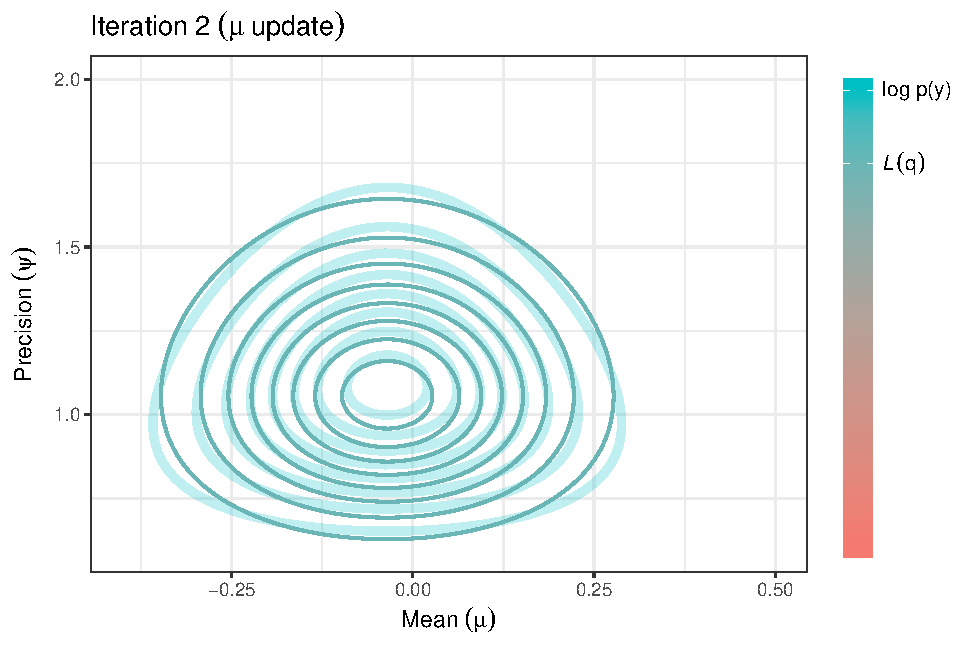
\includegraphics[scale=0.7]{figure/vbupdate_3}
    \end{center}
  } 
  \only<5|handout:5>{
    \begin{center}
      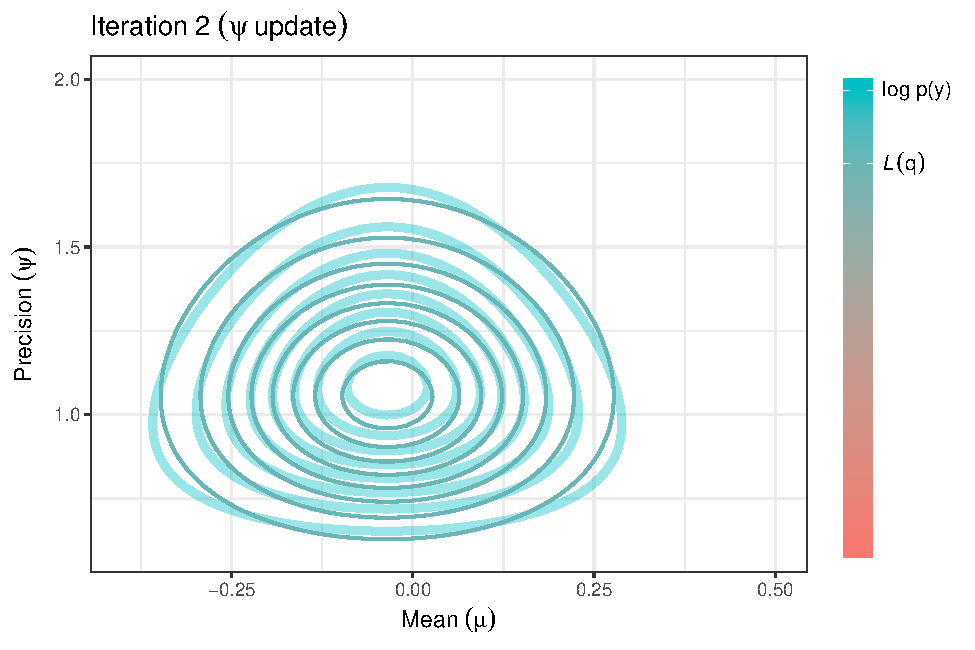
\includegraphics[scale=0.7]{figure/vbupdate_4}
    \end{center}
  } 
  
  \begin{textblock*}{3cm}(.982\textwidth,1.04\textheight)%
    \hyperlink{cavi}{\beamerbutton{back}}      
  \end{textblock*}
\end{frame}
